\documentclass{article}

\usepackage{times}
\usepackage{helvet}
\usepackage{courier}
\usepackage{amsmath,epsfig}
\usepackage{graphicx}
\usepackage{fancyhdr}
\usepackage{times,amsmath,epsfig}
\usepackage{comment}
\usepackage{nccold}
\usepackage{verbatim}
\usepackage[noend]{algorithmic}
\usepackage{color}
\usepackage{url}
\usepackage{float}
\usepackage{alltt}
\usepackage[stable]{footmisc}
\usepackage{subfigure}
\usepackage{epsfig}
\usepackage{amssymb}
\usepackage{amsmath}
\usepackage{amsfonts}
\usepackage{multicol}
\usepackage{caption}
\usepackage{pdflscape}
\usepackage{algorithmic, algorithm}
\usepackage{float}
\usepackage{array}
\usepackage{amsthm}

\DeclareMathOperator*{\argmin}{\arg\!\min}
\DeclareMathOperator*{\argmax}{\arg\!\max}



\def\script#1{\mathcal{#1}}
\def\mS{\script{S}}
\def\mR{\script{R}}

\setlength\parindent{0pt}

\date{}
\title{Discrete Mixture Models}


\begin{document}
	\maketitle

\section{Introduction}

Probability mass function for first bonomial:
\begin{align*}
\phi_1(k_1(i)) = p(k_1(i) | p) = \binom{n}{k_1(i)} p^{k_1(i)} (1-p)^{n - k_1(i)}
\end{align*}

Probability mass function for second binomial:
\begin{align*}
\phi_0(k_1(i)) = p(k_1(i) | q) = \binom{n}{k_1(i)} q^{k_1(i)} (1-q)^{n - k_1(i)}
\end{align*}

Probability mass function for mixture model:
\begin{align*}
p(k_1(1), \cdots, k_1(N) | \alpha, p, q) &= \prod_{i=1}^{N} \left[ \alpha \phi_1(k_1(i)) + (1-\alpha)\phi_0(k_1(i)) \right] \\
&= \prod_{i=1}^{N} \left[ \alpha \binom{n}{k_1(i)} p^{k_1(i)} (1-p)^{n - k_1(i)} + (1-\alpha) \binom{n}{k_1(i)} q^{k_1(i)} (1-q)^{n - k_1(i)}  \right]
\end{align*}



\section{FIM and CRLB}

The derivation for the FIM is included in the appendix. Given equation 1 let the loglikihood be

\begin{align*}
\log L(\mathbb{\theta}) &= \sum_{i=1}^{N} \log \left[ \alpha \binom{n}{k_1(i)} p^{k_1(i)} (1-p)^{n - k_1(i)} + (1-\alpha) \binom{n}{k_1(i)} q^{k_1(i)} (1-q)^{n - k_1(i)}  \right] 
\end{align*}

Then it follows that the Fisher Information Matrix and the Cramer-Rao Lower Bound are

\begin{align*}
FIM &= -\mathrm{E} \left[\frac{d^2 \log p}{d^2\mathbb{\theta}}\right] \\
CRLB &= FIM^{-1}
\end{align*}

The derivations for the derivatives are included in the appendix. When doing the derivations we define

\begin{align*}
P(k | p, n) &= \binom{n}{k}p^{k}(1 - p)^{n - k} \\
P'(k | p, n) &= \frac{dP}{dp} = \binom{n}{k}\left[kp^{k - 1}(1 - p)^{n - k} + (n - k)p^{k}(1 - p)^{n - k - 1}\right]\\
P"(k | p, n) &= \frac{d^2P}{d^2p} = \binom{n}{k}\left[k(k - 1)p^{k - 2}(1 - p)^{n - k} + 2k(n - k)p^{k - 1}(1 - p)^{n - k - 1} + (n - k)(n - k - 1)p^k(1 - p)^{n - k - 2}\right]\\
\end{align*}

The Fisher information matrix is then:

\begin{align*}
-E\begin{bmatrix}\frac{\delta^2\log(L(\mathbb{\theta})}{{\delta\theta}^2}\end{bmatrix} &= -N * E\begin{bmatrix}
F_{\alpha\alpha} F_{\alpha p} F_{\alpha q} \\
F_{\alpha p} F_{pp} F_{pq} \\
F_{\alpha q} F_{pq} F_{qq} \\
\end{bmatrix}
\end{align*}

Where

\begin{align*}
F_{\alpha\alpha} &= \frac{\partial^2L(\mathbb{\theta})}{\partial\alpha^2} = \frac{(P(k | p, n) - P(k | q, n))^2}{(\alpha P(k | p, n) + (1 - \alpha) P(k | q, n))^2} \\
F_{\alpha p} &= \frac{\partial^2L(\mathbb{\theta})}{\partial\alpha\partial p} = \frac{P'(k | p, n)P(k | q, n)}{(\alpha P(k | p, n) + (1 - \alpha) P(k | q, n))^2} \\
F_{\alpha q} &= \frac{\partial^2L(\mathbb{\theta})}{\partial\alpha\partial q} = \frac{-P(k | p, n)P'(k | q, n)}{(\alpha P(k | p, n) + (1 - \alpha) P(k | q, n))^2} \\
F_{pp} &= \frac{\partial^2L(\mathbb{\theta})}{\partial p^2} = \frac{\alpha^2P"(k | p, n)P(k | p, n) + \alpha(1 - \alpha)P"(k | p, n)P(k | q, n) - \alpha^2P(k | p, n)^2}{(\alpha P(k | p, n) + (1 - \alpha) P(k | q, n))^2} \\
F_{pq} &= \frac{\partial^2L(\mathbb{\theta})}{\partial p\partial q} = \frac{-\alpha(1 - \alpha)P'(k | p, n)P'(k | p, n)}{(\alpha P(k | p, n) + (1 - \alpha) P(k | q, n))^2} \\
F_{qq} &= \frac{\partial^2L(\mathbb{\theta})}{\partial q^2} = \frac{\alpha(1 - \alpha)P"(k | q, n)P(k | p, n) + (1 - \alpha)^2P"(k | q, n)P(k | q, n) - (1 - \alpha)^2P'(k | q, n)^2}{(\alpha P(k | p, n) + (1 - \alpha) P(k | q, n))^2}
\end{align*}

\section{Maximum Likelihood and Expectation-Maximization}

\subsection{Maximum Likelihood Equations}
Given Equation \ref{main_pmf}, let the likelihood be
\begin{align*}
L(\mathbb{\theta}) = p(k_1(1), \cdots, k_1(N) | \mathbb{\theta})\ 
\end{align*}
Then, the log-likelihood is
\begin{align*}
\log L(\mathbb{\theta}) &= \sum_{i=1}^{N} \log \left[ \alpha \binom{n}{k_1(i)} p^{k_1(i)} (1-p)^{n - k_1(i)} + (1-\alpha) \binom{n}{k_1(i)} q^{k_1(i)} (1-q)^{n - k_1(i)}  \right] 
\end{align*}

The maximum log-likelihood is given by
\begin{align*}
\hat{\theta} = \argmax_{\theta} \log L(\mathbb{\theta})
\end{align*}
Therefore, the maximum likelihood equations are given by:
%Want to do: $\frac{\delta \log p}{\delta \mathbf{\theta}} = \mathbf{0}$

\begin{align*}
\frac{\delta \log p}{\delta \mathbf{\theta}} &= \begin{bmatrix} 
\sum_{i=1}^{N} \frac{\phi_1(k_1(i)) - \phi_0(k_1(i))}{\alpha \phi_1(k_1(i)) + (1-\alpha)\phi_0(k_1(i))} \\ 
\sum_{i=1}^{N} \frac{\alpha \binom{n}{k_1(i)} \left( k_1(i) p^{k_1(i)-1} (1-p)^{n-k_1(i)} - p^{k_1(i)} (n-k_1(i)) (1-p)^{n-k_1(i)-1} \right) }{\alpha \phi_1(k_1(i)) + (1-\alpha)\phi_0(k_1(i))} \\ 
\sum_{i=1}^{N} \frac{(1-\alpha) \binom{n}{k_1(i)} \left( k_1(i) q^{k_1(i)-1} (1-q)^{n-k_1(i)} - q^{k_1(i)} (n-k_1(i)) (1-q)^{n-k_1(i)-1} \right) }{\alpha \phi_1(k_1(i)) + (1-\alpha)\phi_0(k_1(i))} \end{bmatrix} = \mathbf{0}
\end{align*}

\subsection{EM Algorithm}

Let $\mathbf{k_1} = k_1(1), \cdots, k_1(N)$ be the observed data. 
We introduce membership variables $\mathbf{y} = y(i), \cdots, y(N)$ (hidden data) such that $p(y(i) = c) = \alpha_c$. Because we only have two classes, then 
\begin{align*}
p(y(i) = 1) &= \alpha \\
p(y(i) = 0) &= 1-p(y(i) = 1) = 1 - \alpha
\end{align*}

The joint probability mass function is given by:
\begin{align*}
p(\mathbf{k_1}, \mathbf{y} | \theta ) &= \prod_{i=1}^{N} p(k_1(i), y(i) | \theta ) \\
&= \prod_{i=1}^{N} p(k_1(i) | y(i) ) p(y(i) | \theta )  \\
&= \prod_{i=1}^{N} \prod_{l=1}^{M} (\phi_l(k_1(i) \alpha_l)) ^ {I(y(i)=l)}
\end{align*}

Let $Q$ be an auxiliary function such that
\begin{align*}
Q(\theta, \theta') &= \mathrm{E} \left[ \log p(\mathbf{k_1}, \mathbf{y} | \theta ) | \mathbf{k_1}, \theta' \right] \\
&= \mathrm{E} \left[ \sum_{i=1}^{N} \sum_{l=1}^{M} I(y(i)=l) (\log \phi_l(k_1(i)) + \log \alpha_l) | \mathbf{k_1}, \theta' \right] \\
&= \sum_{i=1}^{N} \sum_{l=1}^{M} \mathrm{E} \left[ I(y(i)=l) | \mathbf{k_1}, \theta' \right] (\log \phi_l(k_1(i)) + \log \alpha_l)  \\
&= \sum_{i=1}^{N} \sum_{l=1}^{M} p(y(i) = c | k_1(i), \theta') (\log \phi_l(k_1(i)) + \log \alpha_l)
\end{align*}

In the E-step of the EM algorithm, we compute $p(y(i) = c | k_1(i), \theta')$. 
In our case of $M=2$ the E-step is given by:
\begin{align*}
p(y(i) = 1 | k_1(i), \mathbf{\theta'}) &= \frac{\alpha \binom{n}{k_1(i)} p^{k_1(i)} (1-p)^{n-k_1(i)}}{\alpha \binom{n}{k_1(i)} p^{k_1(i)} (1-p)^{n-k_1(i)} + (1-\alpha) \binom{n}{k_1(i)} q^{k_1(i)} (1-q)^{n-k_1(i)}} \\
p(y(i) = 0 | k_1(i), \mathbf{\theta'}) &= \frac{(1-\alpha) \binom{n}{k_1(i)} q^{k_1(i)} (1-q)^{n-k_1(i)}}{\alpha \binom{n}{k_1(i)} p^{k_1(i)} (1-p)^{n-k_1(i)} + (1-\alpha) \binom{n}{k_1(i)} q^{k_1(i)} (1-q)^{n-k_1(i)}}
\end{align*}

In the M-step, we compute
\begin{align*}
\theta^{k+1} &= \argmax_\theta Q(\theta, \theta^{k}) \\
&= \argmax_\theta \sum_{i=1}^{N} \sum_{l=1}^{M} p(y(i) = l | k_1(i), \theta^{k}) (\log \phi_l(k_1(i)) + \log \alpha_l)
\end{align*}
In our case of $M=2$, we have
\begin{align*}
\theta^{k+1} &= \argmax_\theta \sum_{i=1}^{N} [ p(y(i) = 1 | k_1(i), \theta^{k}) (\log \phi_1(k_1(i)) + \log \alpha) + \\
& \quad \quad \quad \quad \quad \quad \quad p(y(i) = 0 | k_1(i), \theta^{k}) (\log \phi_0(k_1(i)) + \log (1-\alpha)) ]
\end{align*}

We first maximize $\alpha$. Using Lagrangiang, we get
\begin{align*}
L &= \sum_{i=1}^{N} \sum_{l=1}^{M} p(y(i) = c | k_1(i), \theta^{k}) (\log \alpha_l) + \lambda(\sum_{l=1}^{M} \alpha_l - 1)
\end{align*}
Then, taking the derivative
\begin{align*}
\frac{\delta L}{\delta \alpha} &= \sum_{i=1}^{N} \sum_{l=1}^{M} p(y(i) = c | k_1(i), \theta^{k}) \frac{1}{\alpha_l} + \lambda &= 0
\alpha_l &= -\frac{1}{\lambda} 
\end{align*}


To maximize $p$, we get:
\begin{align*}
p^{k+1} &= \argmax_p \sum_{i=1}^{N}  p(y(i) = 1 | k_1(i), \theta^{k}) \log \phi_1(k_1(i)) \\
&= \argmax_p \sum_{i=1}^{N}  p(y(i) = 1 | k_1(i), \theta^{k}) \log \binom{n}{k_1(i)} p^{k_1(i)} (1-p)^{n-k_1(i)}  \\
&= \argmax_p \sum_{i=1}^{N}  p(y(i) = 1 | k_1(i), \theta^{k}) (\log n! - \log k_1(i)! - \log (n-k_1(i))! + k_1(i) \log p + (n-k_1(i)) \log (1-p))
\end{align*}
Taking the derivative and making equal to 0:
\begin{align*}
\frac{\delta}{\delta p} &= \sum_{i=1}^{N}  p(y(i) = 1 | k_1(i), \theta^{k}) \left( \frac{k_1(i)}{p} + \frac{n-k_1(i)}{1-p} \right) \\
&= \sum_{i=1}^{N}  p(y(i) = 1 | k_1(i), \theta^{k}) \left( \frac{k_1(i)(1-p) - (n-k_1(i))p}{p(1-p)}
\right) \\
&= \sum_{i=1}^{N}  p(y(i) = 1 | k_1(i), \theta^{k}) \left( \frac{k_1(i)- k_1(i)p - np +k_1(i)p}{p(1-p)} \right) \\
&= \sum_{i=1}^{N}  p(y(i) = 1 | k_1(i), \theta^{k}) \left( \frac{k_1(i)- np}{p(1-p)} \right) \\
&= \frac{1}{p(1-p)} \sum_{i=1}^{N} p(y(i) = 1 | k_1(i), \theta^{k}) k_1(i) - \frac{1}{p(1-p)} \sum_{i=1}^{N} p(y(i) = 1 | k_1(i), \theta^{k}) np \\
&= 0 \\
\end{align*}
Therefore, the value that maximizes $p$ is
\begin{align*}
p^{k+1} = \frac{\sum_{i=1}^{N} p(y(i) = 1 | k_1(i), \theta^{k}) k_1(i)}{n \sum_{i=1}^{N} p(y(i) = 1 | k_1(i), \theta^{k})}
\end{align*}
To maximize $q$, we take a similar derivation from the one taken for $p$. Therefore, the value that maximizes $q$ is
\begin{align*}
q^{k+1} &= \frac{\sum_{i=1}^{N} p(y(i) = 0 | k_1(i), \theta^{k}) k_1(i)}{n \sum_{i=1}^{N} p(y(i) = 0 | k_1(i), \theta^{k})}
\end{align*}


Then, we get:
\begin{align*}
\alpha_1^{k+1} &= \alpha^{k+1} = \frac{1}{N} \sum_{i=1}^{N} p(y(i) = 1 | k_1(i), \theta^{k}) \\
\alpha_0^{k+1} &= 1 - \alpha^{k+1} \\
p^{k+1} &= \frac{\sum_{i=1}^{N} p(y(i) = 1 | k_1(i), \theta^{k}) k_1(i)}{n \sum_{i=1}^{N} p(y(i) = 1 | k_1(i), \theta^{k})} \\
q^{k+1} &= \frac{\sum_{i=1}^{N} p(y(i) = 0 | k_1(i), \theta^{k}) k_1(i)}{n \sum_{i=1}^{N} p(y(i) = 0 | k_1(i), \theta^{k})}
\end{align*}


\begin{figure}[!htbp]
	\centering
	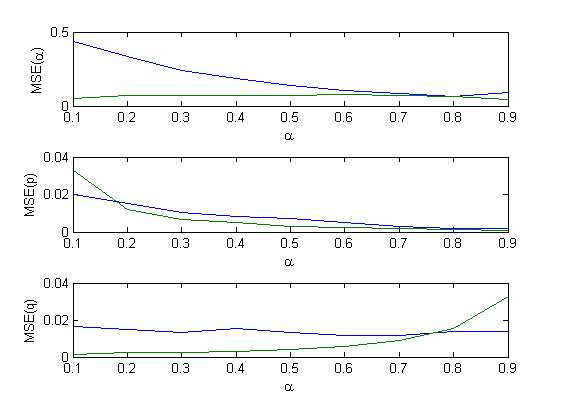
\includegraphics[width=\columnwidth]{images/EM_plot.png} %height=1.7in,
	\vspace{-1pt}
	\caption{CRLB (green) vs EM (blue).}
	\vspace{-2pt}
	\label{figure:crlb-em}
\end{figure}


\section{Method of Moments}


\end{document}

